\documentclass{beamer}
\begin{document}

\title[Introduction to Command-Line]{Introduction to the Command-Line}
\author[Z. Latta]{Zach Latta}
\date[September 2013]{September 25, 2013}

\frame{\titlepage}

\frame{\frametitle{Fundamentals}
  \begin{description}
    \item {\bfseries ls} \hfill \\
      List files and directories in the current directory.
    \item {\bfseries cd [dir]} \hfill \\
      Change the current directory to dir.
    \item {\bfseries mkdir [name]} \hfill \\
      Create a new directory with the name specified.
    \item {\bfseries cp [source] [dest]} \hfill \\
      Copy source into dest.
    \item {\bfseries mv [source] [dest]} \hfill \\
      Move source to dest. This can also be used to rename files.
    \item {\bfseries rm [file]} \hfill \\
      Remove file permanently.
    \item {\bfseries man [command]} \hfill \\
      Open manual page for a command.
  \end{description}
}

\frame{\frametitle{Editing Text}
  \begin{description}
    \item {\bfseries nano [filename]} \hfill \\
      Open filename in the nano text editor.
  \end{description}

  \begin{center}
    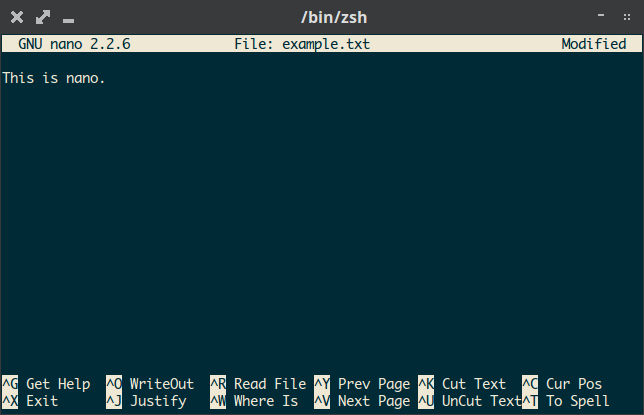
\includegraphics[width=0.75\textwidth]{nano.png}
  \end{center}
}

\frame{\frametitle{Editing Text (cont.)}
  \begin{description}
    \item {\bfseries Ctrl+O} \hfill \\
      Save current document.
    \item {\bfseries Ctrl+W} \hfill \\
      Search in current document.
    \item {\bfseries Ctrl+G} \hfill \\
      Open help.
    \item {\bfseries Ctrl+X} \hfill \\
      Exit nano.
    \item {\bfseries ...and more!} \hfill \\
      The bottom of nano has some common commands. Also read the help.
  \end{description}

}

\end{document}
